\documentclass[11pt,a4paper]{article}
\usepackage[utf8]{inputenc}
\usepackage[T1]{fontenc}
\usepackage[margin=2.2cm]{geometry}
\usepackage{lmodern}
\usepackage{microtype}
\usepackage{amsmath,amssymb}
\usepackage[table]{xcolor}
\usepackage{booktabs}
\usepackage{tabularx}
\usepackage{float}
\usepackage{enumitem}
\usepackage[most]{tcolorbox}
\usepackage{fancyhdr}
\usepackage{needspace}
\usepackage{titlesec}
\usepackage{tikz}
\usetikzlibrary{arrows.meta,positioning,calc,decorations.pathreplacing,shapes.geometric}
\usepackage[colorlinks=true,linkcolor=blue!60!black,urlcolor=blue!60!black]{hyperref}

\setlist[itemize]{nosep,leftmargin=*,topsep=2pt,partopsep=0pt}
\setlist[enumerate]{nosep,leftmargin=*,topsep=2pt,partopsep=0pt}
\widowpenalty=10000
\clubpenalty=10000
\setlength{\parskip}{0.55em}
\setlength{\parindent}{0pt}

% colours
\definecolor{cblue}{HTML}{2B6CB0}
\definecolor{cgreen}{HTML}{2F855A}
\definecolor{cred}{HTML}{C53030}
\definecolor{corange}{HTML}{DD6B20}
\definecolor{cgray}{HTML}{718096}
\definecolor{cpurple}{HTML}{6B46C1}

\titleformat{\section}{\Large\bfseries\color{cblue}}{\thesection}{0.6em}{}
\titleformat{\subsection}{\large\bfseries\color{cblue!80!black}}{\thesubsection}{0.6em}{}

\pagestyle{fancy}
\fancyhf{}
\lhead{\small Paper 03 explained simply}
\rhead{\small Achterhold et al., L4DC 2023}
\cfoot{\small\thepage}
\renewcommand{\headrulewidth}{0.3pt}

% boxes
\newtcolorbox{idea}[1][]{colback=cblue!6,colframe=cblue!70,fonttitle=\bfseries,title={#1},boxrule=0.6pt,arc=2pt,left=6pt,right=6pt,top=4pt,bottom=4pt}
\newtcolorbox{toy}[1][]{colback=corange!7,colframe=corange!80,fonttitle=\bfseries,title={#1},boxrule=0.6pt,arc=2pt,left=6pt,right=6pt,top=4pt,bottom=4pt}
\newtcolorbox{warn}[1][]{colback=cred!6,colframe=cred!75,fonttitle=\bfseries,title={#1},boxrule=0.6pt,arc=2pt,left=6pt,right=6pt,top=4pt,bottom=4pt}
\newtcolorbox{eqbox}[1][]{colback=cgray!8,colframe=cgray!70,fonttitle=\bfseries,title={#1},boxrule=0.6pt,arc=2pt,left=6pt,right=6pt,top=4pt,bottom=4pt}

\newcommand{\vv}{\mathbf{v}}
\newcommand{\pp}{\mathbf{p}}
\newcommand{\ww}{\boldsymbol{\omega}}

\begin{document}
\setcounter{tocdepth}{1}

% ---------------------------------------------------------------- TITLE
\begin{center}
{\LARGE\bfseries\color{cblue} Paper 03, explained from zero}\\[0.6em]
{\large \textit{Black-Box vs.\ Gray-Box: A Case Study on Learning Table Tennis Ball Trajectory Prediction with Spin and Impacts}}\\[0.5em]
Jan Achterhold, Philip Tobuschat, Hao Ma, Dieter Buechler, Michael Muehlebach, Joerg Stueckler\\
Max Planck Institute for Intelligent Systems, accepted at L4DC 2023 (arXiv 2305.15189)
\end{center}

\begin{idea}[What this guide is]
This is a slow, step-by-step explanation of one research paper, written for someone who is
\emph{not} used to academic papers. Every symbol is explained the first time it appears. Every
number that comes from the paper is marked as \textbf{(paper)}. Numbers I invented only to
make an idea easier to see are in orange boxes called \textbf{Toy example} and are
\emph{not} from the paper. Red boxes are my own critical comments, so you can tell them apart
from what the authors claim.
\end{idea}

\subsection*{The whole paper in five sentences}
A robot that plays table tennis must know where the ball will be in the next second. Cameras
only give noisy positions, and they sometimes lose the ball. The authors write down the physics
of a flying and bouncing ball, put that physics inside a filter (an \emph{extended Kalman
filter}, EKF), and then let a computer \emph{learn} the unknown numbers of that filter from
recorded data. This mixture of ``known physics'' and ``learned numbers'' is called a
\emph{gray-box} model. It predicted the ball better than two pure neural-network models, and a
real robot arm returned 29 out of 30 balls using it.

\tableofcontents

% ---------------------------------------------------------------- 1
\section{The story in one page}

Imagine you must hit a table tennis ball that flies towards you at several metres per second.
You have well under a second. To hit it you must know \emph{where the ball will be}, not where
it is now. That is a \textbf{prediction} problem.

Three things make it hard:

\textbf{1. Measurements are noisy.} The cameras say ``the ball is here'', but the answer is
always a little wrong, and sometimes the ball is hidden so there is no answer at all.

\textbf{2. The motion is not a straight line.} Gravity pulls the ball down. Air slows it
(drag). Spin bends its path sideways or up/down (the Magnus effect). When it hits the table it
bounces and its speed and spin change.

\textbf{3. Some quantities cannot be seen.} A camera sees position. It does \emph{not} see
the spin, and spin changes the bounce a lot.

The authors' answer is a pipeline (Figure~\ref{fig:pipeline}): measure, filter with a physics
model, then run the physics forward to predict.

\begin{figure}[htbp]
\centering
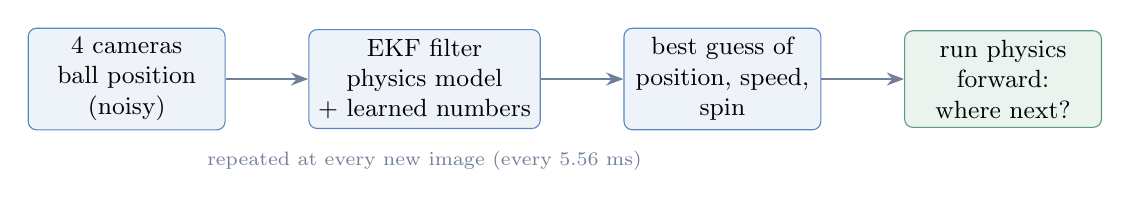
\begin{tikzpicture}[node distance=1.05cm,
  box/.style={draw=cblue!80,fill=cblue!8,rounded corners=3pt,minimum height=1.05cm,minimum width=2.5cm,align=center,font=\small},
  arr/.style={-{Stealth[length=2.2mm]},thick,cgray}]
\node[box] (cam) {4 cameras\\ ball position\\ (noisy)};
\node[box,right=of cam] (filt) {EKF filter\\ physics model\\ + learned numbers};
\node[box,right=of filt] (state) {best guess of\\ position, speed,\\ spin};
\node[box,right=of state,fill=cgreen!10,draw=cgreen!80] (pred) {run physics\\ forward:\\ where next?};
\draw[arr] (cam) -- (filt);
\draw[arr] (filt) -- (state);
\draw[arr] (state) -- (pred);
\node[font=\scriptsize,cgray,below=0.15cm of filt] {repeated at every new image (every 5.56 ms)};
\end{tikzpicture}
\caption{The pipeline of the paper. The robot uses the predicted path to choose where and when to hit.}
\label{fig:pipeline}
\end{figure}

\subsection*{Why not just fit a curve to the points?}
You could fit a smooth curve through the last few measured points. People did this before
(the paper mentions polynomial curves). The problem is that a bounce is a sudden change, and
a curve fitted \emph{before} the bounce does not know about it. A physics model does.

\subsection*{Why not just train a neural network?}
You could feed past positions to a neural network and ask it for future positions. This is
called \textbf{black-box} learning because you do not tell it any physics. It needs a lot of
data and can make strange mistakes. The authors compare against two such networks (RSSM and
TVAE) and their physics-based version wins.

\subsection*{Why ``gray-box''?}
Pure physics is a \textbf{white box} (everything known, nothing learned). A pure neural network is a
\textbf{black box} (nothing known, everything learned). A \textbf{gray box} keeps the physics
\emph{structure} and learns only the numbers we do not know precisely, such as how strongly
the air slows this particular ball.

% ---------------------------------------------------------------- 2
\section{Words you need first}

\begin{table}[htbp]
\centering
\small
\renewcommand{\arraystretch}{1.25}
\begin{tabularx}{\textwidth}{@{}>{\bfseries}p{3.2cm}X@{}}
\toprule
Word & Plain meaning \\
\midrule
State & The list of numbers that describes the ball completely enough to predict its future: where it is, how fast it moves, how it spins, and a few physics constants. \\
Measurement & What the cameras report. Here only the 3D position of the ball centre. \\
Noise & Random error. A measurement is the truth plus a small random error. \\
Filter & A method that combines a model (what should happen) with measurements (what was seen) to get a better guess than either alone. \\
Kalman filter (KF) & The classic filter. It works when the model is a straight-line (linear) relation and the errors are bell-curve shaped (Gaussian). \\
Extended Kalman filter (EKF) & A Kalman filter for curved (nonlinear) models. It pretends the model is a straight line \emph{locally}. \\
Covariance & A table of numbers saying how unsure the filter is about each part of the state. Small numbers mean ``confident''. \\
Process noise ($\mathbf Q$) & How much the filter allows the real ball to differ from the model's prediction, per step. A knob for ``how much do I trust my physics?'' \\
Measurement noise ($\mathbf R$) & How big the camera errors are. A knob for ``how much do I trust the camera?'' \\
Drag & Air resistance. It pushes against the motion. \\
Magnus effect & A spinning ball curves because air flows differently on its two sides. \\
Spin ($\boldsymbol\omega$) & How fast and around which axis the ball rotates. \\
Restitution (bounce) & How much of its speed a ball keeps after hitting a surface. \\
Likelihood & A score for how well a model explains the data. Higher means the data looks less surprising to the model. \\
Black / gray / white box & Learning with no physics / some physics plus learning / only physics. \\
\bottomrule
\end{tabularx}
\caption{Short glossary. Come back to it whenever a word feels unfamiliar.}
\end{table}

% ---------------------------------------------------------------- 3
\section{Step 1: the physics of the flying ball}

When the ball is in the air and not touching anything, the paper says its acceleration is
(equation 1 of the paper):
\begin{equation}
\dot{\vv}(t) \;=\; -k_d\,\|\vv(t)\|\,\vv(t) \;+\; k_m\,\big(\ww(t)\times\vv(t)\big) \;+\; \mathbf g .
\tag{P1}\label{eq:flight}
\end{equation}
\noindent It looks scary, but it has only three parts. Read it as ``change of velocity =
drag + spin-curve + gravity''.

\begin{figure}[htbp]
\centering
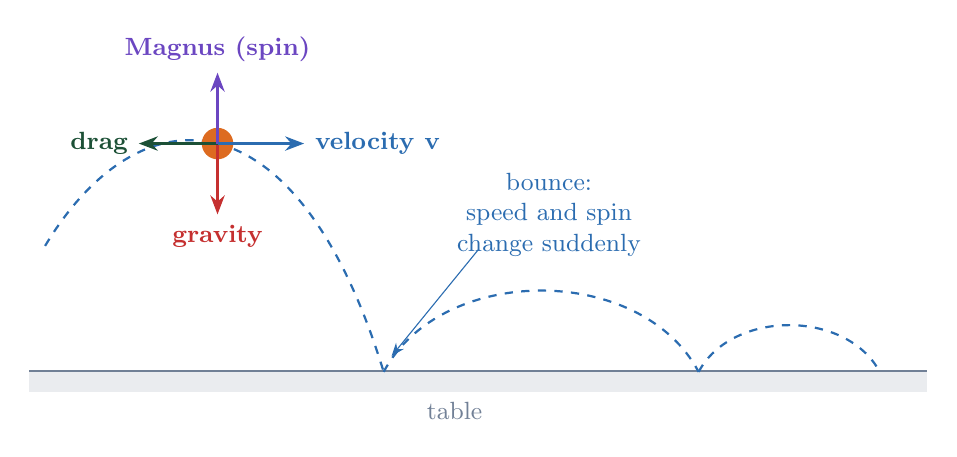
\begin{tikzpicture}[scale=1.0,
  f/.style={-{Stealth[length=2.4mm]},very thick}]
% table
\draw[very thick,cgray] (-0.2,0) -- (11.2,0);
\fill[cgray!15] (-0.2,0) rectangle (11.2,-0.25);
\node[cgray,font=\small] at (5.2,-0.5) {table};
% trajectory
\draw[thick,dashed,cblue] (0,1.6) .. controls (1.2,3.6) and (3.2,3.6) .. (4.3,0);
\draw[thick,dashed,cblue] (4.3,0) to[out=62,in=118] (8.3,0);
\draw[thick,dashed,cblue] (8.3,0) to[out=62,in=118] (10.6,0);
% ball at apex of first arc
\fill[corange] (2.19,2.9) circle (0.2);
% forces
\draw[f,cred] (2.19,2.9) -- ++(0,-0.9) node[below,font=\small\bfseries] {gravity};
\draw[f,cgreen!60!black] (2.19,2.9) -- ++(-1.0,0) node[left,font=\small\bfseries] {drag};
\draw[f,cpurple] (2.19,2.9) -- ++(0,0.9) node[above,font=\small\bfseries] {Magnus (spin)};
\draw[f,cblue] (2.19,2.9) -- ++(1.1,0) node[right,font=\small\bfseries] {velocity $\vv$};
% bounce note
\node[font=\small,align=center,cblue] at (6.4,2.0) {bounce:\\ speed and spin\\ change suddenly};
\draw[-{Stealth},cblue] (5.5,1.55) -- (4.4,0.2);
\end{tikzpicture}
\caption{Forces on the ball in flight (Figure is a drawing, not data). Drag points against the
motion, gravity points down, the Magnus force points sideways to both velocity and spin axis.}
\label{fig:forces}
\end{figure}

\paragraph{Gravity: $\mathbf g=(0,0,-9.802)\ \text{m/s}^2$.}
The ball falls. The third number is negative because $z$ points up. The value 9.802 is the one
used in the paper.

\paragraph{Drag: $-k_d\,\|\vv\|\,\vv$.}
$\|\vv\|$ is the speed (the length of the velocity vector). Multiplying the velocity vector by the
speed again gives something that grows with the \emph{square} of the speed, and the minus sign
makes it push against the motion. The number $k_d$ says how strong the air is for this ball.
It is one of the numbers the computer will learn.

\paragraph{Magnus: $k_m(\ww\times\vv)$.}
The symbol $\times$ is the \emph{cross product}. It builds a vector that is at a right angle to
both the spin axis and the velocity. That is exactly the direction in which a spinning ball
curves. The number $k_m$ says how strong this curving is. It is also learned.

\begin{toy}[Toy example (invented numbers) --- how big is drag?]
Suppose $k_d=0.1$ and the ball flies at $5\ \text{m/s}$. Then the drag deceleration is about
$0.1\times 5\times 5 = 2.5\ \text{m/s}^2$. Compare with gravity, $9.8\ \text{m/s}^2$. Drag is
smaller than gravity but not negligible over a whole second. Double the speed and drag becomes
four times larger. These numbers are \emph{not} from the paper; they only show the scale.
\end{toy}

\paragraph{A trick with squares (important, but easy).}
Physically $k_d$ and $k_m$ must never be negative. Instead of telling the computer
``keep it positive'', the authors store two helper numbers $a_d$ and $a_m$ and define
\begin{equation*}
k_d = a_d^2+\epsilon,\qquad k_m = a_m^2+\epsilon,\qquad \epsilon=0.05\ \text{(paper)}.
\end{equation*}
\noindent A square is never negative, so $k_d$ and $k_m$ can never become negative whatever the
learning does. The small $\epsilon$ keeps them away from exactly zero, which helps the
learning stay stable.

% ---------------------------------------------------------------- 4
\section{Step 2: the bounce}

Equation~\eqref{eq:flight} is valid only in the air. When the ball touches the table, speed and
spin change suddenly. The paper uses a deliberately simple model (equation 2):
\begin{equation}
\begin{pmatrix}\vv^{+}\\ \ww^{+}\end{pmatrix}
\;=\; \mathbf C\begin{pmatrix}\vv^{-}\\ \ww^{-}\end{pmatrix},
\qquad \mathbf C\in\mathbb R^{6\times 6}.
\tag{P2}
\end{equation}
\noindent The minus sign means ``just before the hit'' and the plus sign means ``just after''. The
six numbers before (3 for velocity, 3 for spin) are multiplied by a $6\times6$ table of
numbers $\mathbf C$ to give the six numbers after. $\mathbf C$ is \emph{learned}. The authors
do not write down a bounce formula by hand; they let data decide how a bounce mixes speed and
spin. The price is that this map is linear, which is a simplification of real impacts.

\subsection*{When exactly does the bounce happen?}
The camera images arrive every $\Delta T = 1/180\ \text{s}\approx 5.56\ \text{ms}$ \textbf{(paper)}.
The ball can hit the table \emph{between} two images. The authors compute the exact moment
inside the step. Let $h'$ be the gap between the lowest point of the ball and the table. The ball
reaches the table when
\begin{equation*}
h' + v_z\,t + \tfrac12\,g_z\,t^2 = 0 .
\end{equation*}
\noindent This is a normal quadratic equation. Its positive solution is the time $\Delta_{\text{imp}}$ (the
paper writes it in an equivalent form). The filter then does three things: (1) fly the ball
for $\Delta_{\text{imp}}$, (2) apply $\mathbf C$, (3) fly for the rest of the step.

\begin{toy}[Toy example (invented numbers) --- locating a bounce]
Say the ball is moving down with $v_z=-3\ \text{m/s}$ and its lowest point is $h'=1\ \text{cm}$
above the table. Solve $0.01-3t-4.9t^2=0$. The positive root is $t\approx 0.0033\ \text{s}=3.3\ \text{ms}$.
This is shorter than the 5.56 ms step, so the ball hits the table \emph{inside} this step.
The model flies 3.3 ms, applies the bounce, then flies the remaining $\approx 2.2$ ms.
\end{toy}

\begin{figure}[htbp]
\centering
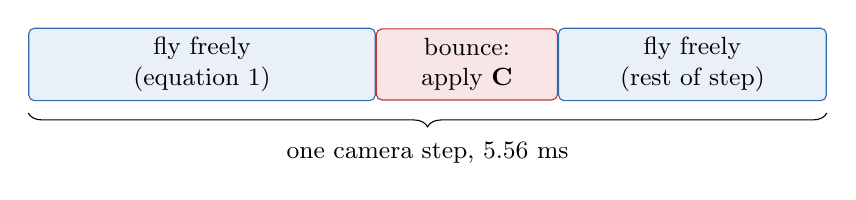
\begin{tikzpicture}[
  seg/.style={draw,rounded corners=2pt,minimum height=0.8cm,font=\small,align=center}]
\node[seg,fill=cblue!10,draw=cblue,minimum width=4.4cm] (a) at (0,0) {fly freely\\ (equation 1)};
\node[seg,fill=cred!12,draw=cred,minimum width=2.3cm,right=0cm of a] (b) {bounce:\\ apply $\mathbf C$};
\node[seg,fill=cblue!10,draw=cblue,minimum width=3.4cm,right=0cm of b] (c) {fly freely\\ (rest of step)};
\draw[decorate,decoration={brace,amplitude=5pt,mirror}] ($(a.south west)+(0,-0.15)$) -- ($(c.south east)+(0,-0.15)$)
  node[midway,below=7pt,font=\small] {one camera step, 5.56 ms};
\end{tikzpicture}
\caption{What happens inside one step when a bounce occurs.}
\end{figure}

% ---------------------------------------------------------------- 5
\section{Step 3: writing the ball as 11 numbers}

A filter needs everything it must remember to be in one list. The paper's \textbf{state} has
11 numbers (equation 3):
\begin{equation}
\mathbf z=(\underbrace{\pp}_{3},\ \underbrace{\vv}_{3},\ \underbrace{\ww}_{3},\ a_d,\ a_m)\in\mathbb R^{11}.
\tag{P3}
\end{equation}

\begin{figure}[htbp]
\centering
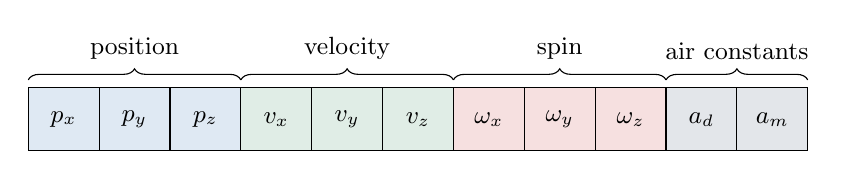
\begin{tikzpicture}[
  c/.style={draw,minimum width=0.9cm,minimum height=0.8cm,font=\small}]
\foreach \i/\t in {0/$p_x$,1/$p_y$,2/$p_z$} \node[c,fill=cblue!15] at (\i*0.9,0) {\t};
\foreach \i/\t in {3/$v_x$,4/$v_y$,5/$v_z$} \node[c,fill=cgreen!15] at (\i*0.9,0) {\t};
\foreach \i/\t in {6/$\omega_x$,7/$\omega_y$,8/$\omega_z$} \node[c,fill=cred!15] at (\i*0.9,0) {\t};
\node[c,fill=cgray!20] at (9*0.9,0) {$a_d$};
\node[c,fill=cgray!20] at (10*0.9,0) {$a_m$};
\draw[decorate,decoration={brace,amplitude=4pt}] (-0.45,0.5) -- (2*0.9+0.45,0.5) node[midway,above=4pt,font=\small] {position};
\draw[decorate,decoration={brace,amplitude=4pt}] (3*0.9-0.45,0.5) -- (5*0.9+0.45,0.5) node[midway,above=4pt,font=\small] {velocity};
\draw[decorate,decoration={brace,amplitude=4pt}] (6*0.9-0.45,0.5) -- (8*0.9+0.45,0.5) node[midway,above=4pt,font=\small] {spin};
\draw[decorate,decoration={brace,amplitude=4pt}] (9*0.9-0.45,0.5) -- (10*0.9+0.45,0.5) node[midway,above=4pt,font=\small] {air constants};
\end{tikzpicture}
\caption{The 11-number state. The camera sees only the first three.}
\end{figure}

Notice something unusual: the physics constants $a_d$ and $a_m$ are \emph{inside the state}.
They are treated as unknown quantities that the filter keeps estimating while the ball flies,
and they are assumed not to change during a flight. The same is true for spin: the model
assumes it stays constant in free flight.

\subsection*{From continuous physics to computer steps}
Equation~\eqref{eq:flight} describes motion at every instant. A computer works in small
jumps. The authors use the simplest rule, \textbf{Euler's method}: new value = old value $+$ step
time $\times$ rate of change. In free flight (equation 4):
\begin{equation}
\begin{aligned}
\pp(t+\Delta_t) &= \pp(t) + \Delta_t\,\vv(t),\\
\vv(t+\Delta_t) &= \vv(t) + \Delta_t\big(-k_d\|\vv\|\vv + k_m(\ww\times\vv)+\mathbf g\big),\\
\ww,\ a_d,\ a_m &\ \text{stay the same.}
\end{aligned}
\tag{P4}
\end{equation}
\noindent In words: move the ball by speed times time, then change the speed by acceleration times
time. Call this whole one-step rule $g_{\text{free}}$. Combine it with the bounce logic of Step~2 and you get
the single ``one step forward'' function of the paper,
$\mathbf z_{n+1}=g(\mathbf z_n)$ (equation 5).

% ---------------------------------------------------------------- 6
\section{Step 4: the filter}

\subsection{The idea of any Kalman filter}
Two sources of information are each a little wrong:
\begin{itemize}
\item the \textbf{model} says ``from where it was, now it should be about here'', with some
uncertainty;
\item the \textbf{camera} says ``it is about there'', with some uncertainty.
\end{itemize}
The filter blends the two. It trusts the more certain source more. After blending, the result is
\emph{more certain than either} source alone. It repeats two steps forever.

\textbf{Predict} (use the model): move the state forward one step. Uncertainty grows, because the
model is not perfect.

\textbf{Correct} (use the measurement): compare what the camera saw with what you predicted,
and shift the guess towards the camera by an amount that depends on how much you trust each.

\begin{toy}[Toy example (invented numbers) --- one correction in one dimension]
Take just the ball's position along one line, in centimetres.

\textbf{Predict:} the model says the ball is at $101.1$ cm, with uncertainty (standard deviation)
$4$ cm, so variance $16$.\\
\textbf{Measure:} the camera says $106$ cm, with uncertainty $3$ cm, so variance $9$.

\textbf{Trust weight (the Kalman gain):} $K=\dfrac{16}{16+9}=0.64$. The model is more
uncertain than the camera, so we lean towards the camera ($64\%$).\\
\textbf{New estimate:} $101.1+0.64\times(106-101.1)=104.2$ cm.\\
\textbf{New uncertainty:} variance $(1-0.64)\times 16=5.76$, standard deviation $2.4$ cm.

The result ($104.2\pm2.4$) is more certain than both inputs ($\pm4$ and $\pm3$).
\end{toy}

\begin{figure}[htbp]
\centering
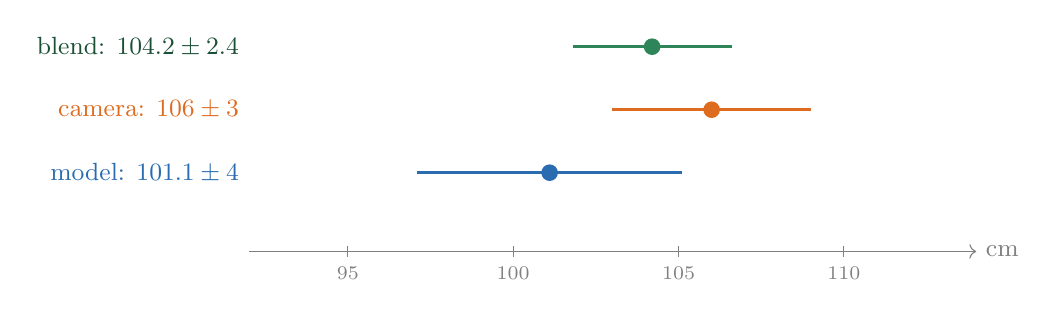
\begin{tikzpicture}[x=0.42cm,y=1cm]
\draw[->,gray] (92,0) -- (114,0) node[right,font=\small] {cm};
\foreach \x in {95,100,105,110} \draw[gray] (\x,0.07) -- (\x,-0.07) node[below,font=\scriptsize] {\x};
\draw[very thick,cblue] (97.1,1.0) -- (105.1,1.0); \fill[cblue] (101.1,1.0) circle (3pt);
\node[font=\small,cblue,left] at (92,1.0) {model: $101.1\pm4$};
\draw[very thick,corange] (103,1.8) -- (109,1.8); \fill[corange] (106,1.8) circle (3pt);
\node[font=\small,corange,left] at (92,1.8) {camera: $106\pm3$};
\draw[very thick,cgreen] (101.8,2.6) -- (106.6,2.6); \fill[cgreen] (104.2,2.6) circle (3pt);
\node[font=\small,cgreen!60!black,left] at (92,2.6) {blend: $104.2\pm2.4$};
\end{tikzpicture}
\caption{The blend sits between the two sources and its bar is the shortest, meaning the most
certain (toy numbers).}
\end{figure}

\subsection{What ``extended'' adds}
The simple Kalman filter needs a straight-line model. The ball's model is curved: drag depends on
speed squared, the cross product mixes components, and the bounce is a jump. The EKF keeps the
same predict-correct recipe but handles the curve by using a \textbf{Jacobian} $\mathbf J$.
The Jacobian is a table of numbers saying: ``if the state changes a tiny bit, how much does the
next state change?'' It is the local straight-line version of the curved model, and the filter
uses it to know how uncertainty travels through one step.

\subsection{The filter equations of the paper, translated}
\begin{eqbox}[Predict step (the paper's text)]
\[
\boldsymbol\mu_{n+1|1:n}=g(\boldsymbol\mu_{n|1:n}),\qquad
\boldsymbol\Sigma_{n+1|1:n}=\mathbf J\,\boldsymbol\Sigma_{n|1:n}\,\mathbf J^{\top}+\mathbf Q .
\]
\textbf{Meaning:} $\boldsymbol\mu$ is the best guess of the 11 numbers; $\boldsymbol\Sigma$ is the $11\times11$ uncertainty table.
First line: push the guess one step forward with the physics. Second line: uncertainty is
carried through the step by $\mathbf J$ and then \emph{increased} by the process noise $\mathbf Q$
($\mathbf Q$ is the ``my physics is not perfect'' knob).
\end{eqbox}

\begin{eqbox}[Correct step (the paper's text)]
\[
\mathbf K=\boldsymbol\Sigma_{n+1|1:n}\mathbf H^{\top}\big(\mathbf H\boldsymbol\Sigma_{n+1|1:n}\mathbf H^{\top}+\mathbf R\big)^{-1},
\]
\[
\boldsymbol\mu_{n+1|1:n+1}=\boldsymbol\mu_{n+1|1:n}+\mathbf K\big(\mathbf m_{n+1}-\mathbf H\boldsymbol\mu_{n+1|1:n}\big),
\qquad
\boldsymbol\Sigma_{n+1|1:n+1}=(\mathbf I-\mathbf K\mathbf H)\boldsymbol\Sigma_{n+1|1:n}.
\]
\textbf{Meaning:} $\mathbf m$ is the camera measurement (3 numbers). $\mathbf H=[\mathbf I_3,\ \mathbf 0_{3\times8}]$
simply says ``the camera sees the first three numbers of the state (the position) and nothing
else''. $\mathbf R$ is the camera-noise table. $\mathbf K$ is the trust weight, exactly the
$0.64$ of the toy example but for a whole table of numbers. The bracket
$(\mathbf m-\mathbf H\boldsymbol\mu)$ is the \emph{surprise}: measurement minus what the filter expected.
\end{eqbox}

\subsection{The two kinds of noise, in this paper}
Process noise: $\mathbf z_{n+1}=g(\mathbf z_n)+\boldsymbol\zeta$ with $\boldsymbol\zeta\sim\mathcal N(\mathbf 0,\mathrm{diag}([\boldsymbol\sigma_q]_+))$,
which is one noise level for each of the 11 numbers. Measurement noise:
$\mathbf m_n=\hat{\mathbf p}_n+\boldsymbol\epsilon$ with $\boldsymbol\epsilon\sim\mathcal N(\mathbf 0,\mathrm{diag}([\boldsymbol\sigma_r]_+))$, one noise level for each of the 3 position axes. The
bracket $[x]_+=\log(1+e^x)+10^{-6}$ is the \emph{softplus}: a smooth function that always returns a positive
number, used again so that noise levels can never be negative.

\subsection{What if the camera loses the ball?}
The paper says the camera system ``occasionally'' cannot give a position (for example because
the ball is hidden). The authors handle this simply: during missing images the filter does
\emph{several predict steps in a row} and corrects only when a measurement finally arrives.
During those steps the uncertainty keeps growing, which is the honest thing to do.

% ---------------------------------------------------------------- 7
\section{Step 5: starting the filter}

A filter needs a first guess. The authors start it at the \textbf{second available measurement}:
\begin{itemize}
\item position = the second measurement $\mathbf m_{\tau(2)}$;
\item velocity = a finite difference: $(\mathbf m_{\tau(2)}-\mathbf m_{\tau(1)})/(\Delta T\,(\tau(2)-\tau(1)))$, which is simply ``distance between the first two points divided by the time between them''. The notation $\tau(n)$ means ``the index of the $n$th available measurement'', needed because some images are missing;
\item the starting uncertainties for position and velocity are \emph{learned numbers}.
\end{itemize}
The two air constants $a_d$ and $a_m$ start from a learned average value with a learned uncertainty.

\subsection{The spin problem, and the paper's trick}
Positions alone barely tell you the spin, and the paper cites earlier works that say the same.
Yet a wrong spin ruins long predictions, especially after a bounce. So where does the initial spin
come from? In this paper the balls are shot by a \textbf{ball launcher}: a machine with three
rubber wheels whose speeds (and aiming angles) are known settings. The authors train a small
neural network that maps the \emph{launcher settings} to the initial spin (and to its uncertainty).
This works only for balls before their first bounce; after a bounce the old relation no longer
holds, so they start the spin at $0$ with a large learned uncertainty.

Two details help understanding. First, the network predicts the spin for a launcher aimed along a
reference direction, and the result is rotated to match the real launch direction. Second, the paper can
recover the spin only \emph{up to a scale factor}: in equation~\eqref{eq:flight} the spin
$\ww$ and the Magnus constant $k_m$ appear as a product, so a bigger $\ww$ with a smaller $k_m$
looks the same. The true spin could be recovered if the ball mass, air density, radius and
a lift coefficient were known.

\begin{warn}[My comment: this part is hard to copy]
The launcher-to-spin trick needs a machine whose settings are known. In a real match there is
none, and in your MuJoCo project the launch settings are also unknown to the estimator.
The idea (use whatever \emph{extra information about the launch} exists) is useful,
but the exact method is specific to this laboratory.
\end{warn}

% ---------------------------------------------------------------- 8
\section{Step 6: teaching the filter}

This is the part that makes the method ``gray-box''. A normal EKF has many numbers that a human
must guess and tune. Here, the computer learns them from data.

\begin{table}[htbp]
\centering
\small
\renewcommand{\arraystretch}{1.2}
\begin{tabularx}{\textwidth}{@{}l X@{}}
\toprule
Learned symbol & What it is \\
\midrule
$\mathbf C$ & the $6\times6$ bounce table \\
$\boldsymbol\sigma_q$ & process noise levels (11 values) \\
$\boldsymbol\sigma_r$ & camera noise levels (3 values) \\
$\boldsymbol\sigma_p,\ \boldsymbol\sigma_v$ & starting uncertainty of position and velocity \\
$\psi_f$ & weights of the launcher-to-spin neural network \\
$\boldsymbol\sigma_\omega,\ \boldsymbol\sigma_{\omega,\text{ai}}$ & starting spin uncertainty (without launch info, and after an impact) \\
$a_d,\ a_m,\ \sigma_{a_d},\ \sigma_{a_m}$ & average starting values and uncertainties of the air constants \\
\bottomrule
\end{tabularx}
\caption{The parameter set $\Psi$ that is learned (from the paper). Everything else is fixed physics.}
\end{table}

\subsection{How can you learn the numbers of a filter?}
Use the idea of ``surprise''. When the filter is about to receive a new measurement, it already has
an expectation of what it will see and how uncertain that expectation is. If the real
measurement is far from the expectation \emph{given that uncertainty}, the filter is
surprised, which means the numbers are bad. If measurements keep arriving close to expectations,
the numbers are good. Mathematically the paper adds up, over a recorded trajectory, the log
probability that the filter gave to what actually happened:
\begin{equation}
\log p(\mathbf m_{3:N}\mid\mathbf m_1,\mathbf m_2,\Psi)
=\sum_{n=3}^{N}\log\mathcal N\big(\mathbf m_n;\ \boldsymbol\mu_{n|1:n-1},\ \boldsymbol\Sigma_{n|1:n-1}\big).
\tag{P7}\label{eq:loglik}
\end{equation}
\noindent The learning procedure changes $\Psi$ so that this number becomes as large as possible. The
trajectory is conditioned on the first two measurements because those are used to start the filter.

\begin{figure}[htbp]
\centering
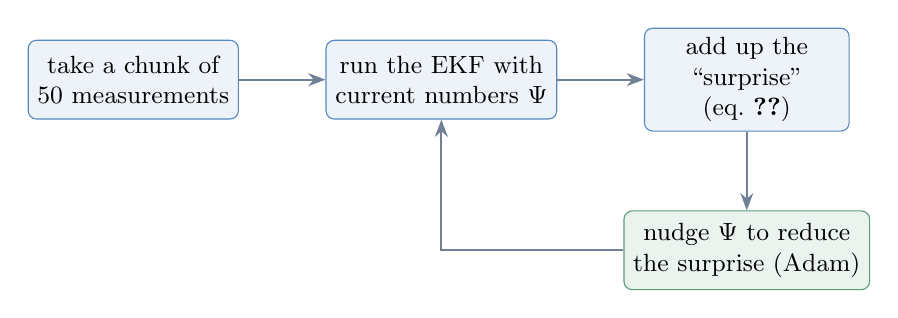
\begin{tikzpicture}[node distance=1.1cm,
  box/.style={draw=cblue!80,fill=cblue!8,rounded corners=3pt,minimum height=1cm,minimum width=2.6cm,align=center,font=\small},
  arr/.style={-{Stealth[length=2.2mm]},thick,cgray}]
\node[box] (a) {take a chunk of\\ 50 measurements};
\node[box,right=of a] (b) {run the EKF with\\ current numbers $\Psi$};
\node[box,right=of b] (c) {add up the\\ ``surprise''\\ (eq.~\ref{eq:loglik})};
\node[box,below=1.0cm of c,fill=cgreen!10,draw=cgreen!80] (d) {nudge $\Psi$ to reduce\\ the surprise (Adam)};
\draw[arr] (a) -- (b); \draw[arr] (b) -- (c); \draw[arr] (c) -- (d); \draw[arr] (d.west) -| (b.south);
\end{tikzpicture}
\caption{The learning loop. It repeats over many chunks. Because the EKF is built from smooth
operations, the computer can compute how a tiny change of each number changes the surprise, and
use that to improve all numbers at once.}
\end{figure}

\subsection{The details of the training (all from the paper)}
\textbf{Chunks:} a long trajectory is cut into overlapping pieces of $N=50$ consecutive
measurements, and a random chunk is chosen each time (uniform probability). \textbf{Optimiser:} Adam,
learning rate $5\cdot10^{-3}$, batch size 64 chunks. Short chunks make each pass cheap: the cost grows only
linearly with the chunk length.

\textbf{What you gain:} ``no tedious tuning of initial, transition, and observation covariances
is required'' (the authors' conclusion). \textbf{What you pay:} you need recorded trajectories, and the
result is only as good as that data.

% ---------------------------------------------------------------- 9
\section{The experiment}

\subsection{The set-up}
A ball launcher shoots table tennis balls towards a robot arm. The ball position is measured by
\textbf{four RGB cameras} at 180 images per second. The launcher was placed at six positions.
One is called \emph{default} (used for training and testing) and five are \emph{unseen} (used only for testing).
The robot arm is a 4-degree-of-freedom arm driven by pairs of artificial pneumatic muscles; it was used only for
the final return test.

\begin{figure}[htbp]
\centering
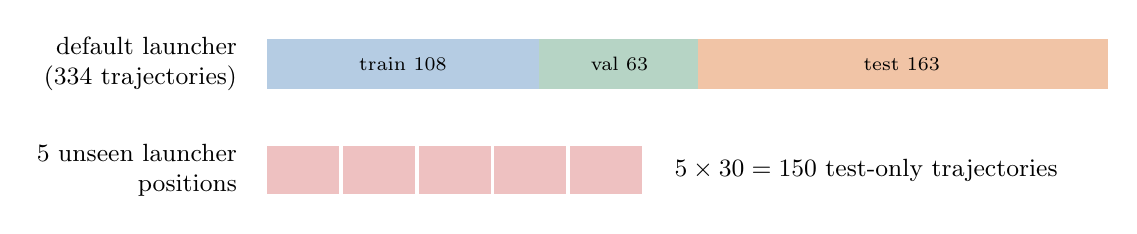
\begin{tikzpicture}[x=0.032cm,y=0.9cm]
\fill[cblue!35] (0,2.4) rectangle (108,3.1); \node[font=\scriptsize] at (54,2.75) {train 108};
\fill[cgreen!35] (108,2.4) rectangle (171,3.1); \node[font=\scriptsize] at (140,2.75) {val 63};
\fill[corange!40] (171,2.4) rectangle (334,3.1); \node[font=\scriptsize] at (252,2.75) {test 163};
\node[anchor=east,font=\small,align=right] at (-8,2.75) {default launcher\\ (334 trajectories)};
\foreach \i in {0,...,4} {\fill[cred!30,draw=white] (\i*30,0.9) rectangle (\i*30+29,1.6);}
\node[anchor=east,font=\small,align=right] at (-8,1.25) {5 unseen launcher\\ positions};
\node[anchor=west,font=\small] at (158,1.25) {$5\times30=150$ test-only trajectories};
\end{tikzpicture}
\caption{The data of the paper: 334 trajectories from the default launcher (108 / 63 / 163),
and $5\times30=150$ test-only trajectories from unseen launcher positions.}
\end{figure}

\subsection{Data augmentation: why it was necessary}
The training data came from only one launcher position, so it covers only certain directions. To
help the model on the unseen positions, each training trajectory was \emph{rotated by a random angle
around the vertical axis} (at its lowest point) $19$ times, creating 19 extra copies. This is
a smart cheap trick: physics does not care in which compass direction you shoot. The paper reports
that without this augmentation the EKF generalises worse to the unseen launcher positions.

\subsection{The two competitors}
\textbf{RSSM} (Hafner et al., 2019), a neural network that learns a hidden ``latent'' state and
predicts forward in it; trained for 100,000 steps. \textbf{TVAE} (G\'omez-Gonz\'alez et al., 2020), a variational
auto-encoder over whole trajectories (length 250). Both are black boxes: no
physics inside. RSSM could optionally receive the same launch information as the EKF; TVAE did not (see the paper's Figure 5a).

\subsection{How they measured success}
For each test trajectory the filter runs until \textbf{one second before the end}, then the model
predicts the last second without seeing any more measurements. The error is the \emph{largest distance} among the last
five predicted/measured pairs. Ten models were trained independently for each method, so the
spread over those ten models is shown.

\begin{figure}[htbp]
\centering
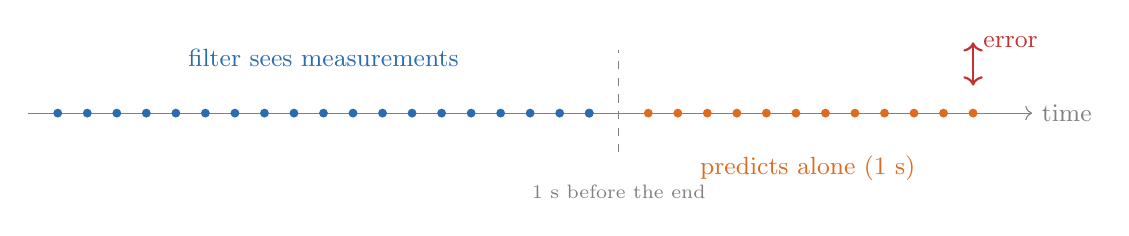
\begin{tikzpicture}[x=0.075cm,y=1cm]
\draw[->,gray] (0,0) -- (170,0) node[right,font=\small] {time};
\foreach \x in {5,10,...,95} \fill[cblue] (\x,0) circle (1.6pt);
\fill[cblue] (95,0) circle (1.6pt);
\foreach \x in {105,110,...,160} \fill[corange] (\x,0) circle (1.6pt);
\draw[<->,cred,thick] (160,0.35) -- (160,0.9) node[right,font=\small] {error};
\draw[dashed,gray] (100,-0.5) -- (100,0.8);
\node[font=\small,cblue,align=center] at (50,0.7) {filter sees measurements};
\node[font=\small,corange,align=center] at (132,-0.7) {predicts alone (1 s)};
\node[font=\scriptsize,gray] at (100,-1.0) {1 s before the end};
\end{tikzpicture}
\caption{How prediction quality is tested: the final prediction is compared with the real ball
position (the last five pairs are compared and the worst one counts).}
\end{figure}

\Needspace{14\baselineskip}
\subsection{What they found}
\begin{table}[htbp]
\centering
\small
\renewcommand{\arraystretch}{1.25}
\begin{tabularx}{\textwidth}{@{}p{4.3cm}X@{}}
\toprule
Question & Answer (paper) \\
\midrule
Does the gray-box EKF beat the black boxes? & Yes: in every setting tested it had lower prediction error than RSSM and TVAE. \\
Does the rotation augmentation matter? & Yes, especially for the unseen launcher positions. \\
Does launcher information help? & Yes, ``drastically'': predicting the spin from launcher settings reduced the 1-second prediction error much more than estimating the spin from positions alone. \\
How big is the error in numbers? & On the unseen launcher positions with launch information, the \textbf{median} 1-second prediction error was \textbf{10.3 cm}; the worst example was 39.3 cm and the best 0.6 cm (their Figure 6). \\
Is the learned spin physically believable? & The network's spin correlates highly with a simple spin model built from the wheel speeds (their equation 8 and Figure 7). \\
Does it work on a real robot? & The arm returned \textbf{29 of 30} balls, re-planning the hit each time the filter updated. \\
\bottomrule
\end{tabularx}
\caption{Summary of the results. Most of them are shown only as plots in the paper, so I only quote the numbers that are written in the text.}
\end{table}

% ---------------------------------------------------------------- 10
\section{Critical reading: what is strong and what is weak}

\begin{idea}[Strengths]
(1) The physics structure keeps the model interpretable: you can read $k_d$, $\mathbf C$ and the noise
levels. (2) Learning the filter numbers removes hand-tuning. (3) It uses little data (108 training
trajectories) because most knowledge is already in the equations. (4) It was tested on a real
robot, not only offline. (5) It handles missing measurements simply and honestly.
\end{idea}

\begin{warn}[Weak points and things to double-check]
\textbf{A. An arithmetic slip.} The abstract and Section 4.4 say 29 of 30 returned balls is
$97.7\%$. But $29/30=96.7\%$. The count (29 of 30) is what to trust; I would quote ``29/30'' and not $97.7\%$.

\textbf{B. Only black boxes as rivals.} The comparisons are against RSSM and TVAE. There is no
comparison against a classic hand-tuned EKF or UKF. So the paper shows ``physics plus learning beats pure
learning'', not ``learned filter numbers beat carefully tuned ones''.

\textbf{C. The metric is demanding.} The error is the \emph{largest} of the last five
differences, so it measures worst-case behaviour near the end. That is fair for catching, but it is
not an average error.

\textbf{D. Mostly plots.} Many comparisons are only in figures, so exact numbers cannot be quoted
from the text, other than the median 10.3 cm.

\textbf{E. Bounce and linearisation (my own observation).} The one-step function $g$ contains an
if-statement (bounce or no bounce). The EKF's Jacobian is a local straight-line approximation, and
a bounce is a jump. The paper does not discuss how this is treated at the exact bounce step, so I would test it carefully in your own simulation rather
than assume it works.

\textbf{F. Narrow world.} One table, one ball type, one launcher, a short flight. Whether the
learned numbers transfer to other balls or surfaces is not shown.
\end{warn}

% ---------------------------------------------------------------- 11
\section{What we take for our MuJoCo project}

Your ball slides on a floor and may have friction and bounces. Compare the two situations:

\begin{table}[htbp]
\centering
\small
\renewcommand{\arraystretch}{1.25}
\begin{tabularx}{\textwidth}{@{}p{3.3cm}XX@{}}
\toprule
 & Table-tennis paper & Your project \\
\midrule
Motion in the air & drag + Magnus + gravity & none: the ball stays on the floor, so replace this by \textbf{friction} (speed slowly decreases) \\
Contact event & table bounce (matrix $\mathbf C$) & wall or obstacle bounce; restitution coefficient \\
Spin & hidden, important & probably unimportant at first (you can start without spin and add it later if needed) \\
Measurement & 3D position from 4 RGB cameras & 3D position from a depth camera, with range-dependent noise \\
Training data & 334 real trajectories & unlimited simulated trajectories in MuJoCo \\
\bottomrule
\end{tabularx}
\caption{How the paper maps onto your project.}
\end{table}

\textbf{A first design inspired by this paper (to discuss with me, not final):}
\begin{enumerate}
\item State: ball position (2--3 numbers), velocity (2--3 numbers), and one or two physics constants
(friction coefficient, restitution) --- the same ``put the constants inside the state'' idea.
\item Model: constant-speed motion with a friction term, plus a bounce rule when the ball touches something.
\item Filter: an EKF with the predict-correct equations above, including ``predict-only'' steps when the arm hides the ball.
\item Learn the noise tables and the bounce parameters from simulated trajectories by maximising equation~\eqref{eq:loglik}.
\item Evaluate the same way: filter until a chosen time, predict the rest, measure the final error, and finally feed the estimate to the planners and measure catch success.
\end{enumerate}

% ---------------------------------------------------------------- 12
\section{Test yourself}

\begin{enumerate}[label=\textbf{Q\arabic*.}]
\item \emph{Why is the filter's uncertainty bigger after the predict step than before it?}\\
Because the model is not perfect; $\mathbf Q$ adds uncertainty at every step.
\item \emph{In the toy example, why did the camera get weight $0.64$ and the model only $0.36$?}\\
The camera was the more certain source (standard deviation 3 vs 4).
\item \emph{Why are $a_d$ and $a_m$ squared?}\\
So that the drag and Magnus constants cannot become negative.
\item \emph{Why does the paper need ``spin from launcher settings''?}\\
Positions hardly reveal spin, and a wrong spin makes long predictions bad.
\item \emph{What is learned and what is fixed?}\\
Learned: bounce table, noise levels, starting uncertainties, air constants, the spin network. Fixed: the shape of the physics equations.
\item \emph{Why were the training trajectories rotated?}\\
Physics is the same in every compass direction, so rotated copies teach the model about launch directions it never saw.
\item \emph{What does the number 10.3 cm mean?}\\
The median error of the prediction one second ahead, on the unseen launcher positions with launch information.
\item \emph{What is ``29 of 30''?}\\
The number of balls the real robot arm returned using the filter's predictions (the paper's printed $97.7\%$ should read $96.7\%$).
\end{enumerate}

% ---------------------------------------------------------------- APPENDIX
\appendix
\section{Equation cheat sheet}

\begin{eqbox}[All the main equations in one place]
\textbf{Flight:} $\dot{\vv}=-k_d\|\vv\|\vv+k_m(\ww\times\vv)+\mathbf g,\quad \mathbf g=(0,0,-9.802)$\\[2pt]
\textbf{Constants:} $k_d=a_d^2+\epsilon,\ k_m=a_m^2+\epsilon,\ \epsilon=0.05$\\[2pt]
\textbf{Bounce:} $(\vv^+,\ww^+)=\mathbf C\,(\vv^-,\ww^-)$, $\mathbf C\in\mathbb R^{6\times6}$\\[2pt]
\textbf{State:} $\mathbf z=(\pp,\vv,\ww,a_d,a_m)\in\mathbb R^{11}$, step $\Delta T=1/180\ \text{s}$\\[2pt]
\textbf{Noise:} $\mathbf z_{n+1}=g(\mathbf z_n)+\boldsymbol\zeta$, $\ \mathbf m_n=\hat{\mathbf p}_n+\boldsymbol\epsilon$, $\ [x]_+=\log(1+e^x)+10^{-6}$\\[2pt]
\textbf{Predict:} $\boldsymbol\mu^-=g(\boldsymbol\mu),\ \boldsymbol\Sigma^-=\mathbf J\boldsymbol\Sigma\mathbf J^\top+\mathbf Q$\\[2pt]
\textbf{Correct:} $\mathbf K=\boldsymbol\Sigma^-\mathbf H^\top(\mathbf H\boldsymbol\Sigma^-\mathbf H^\top+\mathbf R)^{-1}$, $\ \boldsymbol\mu=\boldsymbol\mu^-+\mathbf K(\mathbf m-\mathbf H\boldsymbol\mu^-)$, $\ \boldsymbol\Sigma=(\mathbf I-\mathbf K\mathbf H)\boldsymbol\Sigma^-$, $\ \mathbf H=[\mathbf I_3\ \mathbf 0]$\\[2pt]
\textbf{Learning:} maximise $\sum_n\log\mathcal N(\mathbf m_n;\boldsymbol\mu_{n|1:n-1},\boldsymbol\Sigma_{n|1:n-1})$ over chunks of 50; Adam, lr $5\cdot10^{-3}$, batch 64
\end{eqbox}

\section{Where each part is in the paper}

\begin{table}[htbp]
\centering
\small
\renewcommand{\arraystretch}{1.2}
\begin{tabularx}{\textwidth}{@{}l X@{}}
\toprule
Paper section & Content (this guide) \\
\midrule
1 Introduction, 2 Related work & the story, black / gray / white box (Section 1) \\
3.1 Physical model & flight and bounce (Sections 3, 4) \\
3.2 Discrete-time model & 11-number state, Euler steps, impact timing (Sections 4, 5) \\
3.3 EKF & predict, correct, missing data, initialisation, learning (Sections 6, 7, 8) \\
4.1 Set-up, launcher, data & experiment set-up, augmentation (Section 9) \\
4.2 Prediction performance & competitors, metric, results (Section 9) \\
4.3 Spin evaluation & spin check, scale ambiguity (Sections 7, 9) \\
4.4 Return performance & 29 of 30 balls (Section 9) \\
5 Conclusion & strengths (Section 10) \\
\bottomrule
\end{tabularx}
\end{table}

\end{document}
